%%%%%%%%%%%%%%%%%%%%%%%%%%%%%%%%%%%%%%%%%%%%%%%%%%%
%% Conceptions et spécification des besoins
%%%%%%%%%%%%%%%%%%%%%%%%%%%%%%%%%%%%%%%%%%%%%%%%%%%
\section{Conceptions et spécification des besoins}
\addcontentsline{toc}{subsection}{Introduction}
\subsection*{Introduction}
Ce chapitre est voué à fournir une conception détaillée du portail Arkevia (le portail existant), afin d'appréhender son mode de fonctionnement et de bien cerner les besoins et exigences liés au sujet. Nous poursuivons cette conception par l'élaboration des besoins, des contraintes, et des méthodologies et solutions préconisées.
\subsection{Étude conceptuelle du système existant}
L'objectif de cette première section est de mener une étude conceptuelle approfondie du fonctionnement du système.
\subsubsection{Méthodologie de conception}
L’utilisation de la modélisation conceptuelle dans le développement des systèmes d’information permet de prendre en compte les besoins des applications d’une façon plus adéquate et de présenter d’une manière abstraite certains aspects des systèmes physiques et humains.\\

Afin de modéliser et décrire les différents aspects de notre système, nous utiliserons le langage graphique de modélisation unifié UML 2.0.\\
UML est un langage formel et normalisé en termes de modélisation objet. Son indépendance par rapport aux langages de programmation, aux domaines d’application et son caractère polyvalent ont fait de lui un langage universel. Il fournit un moyen astucieux permettant de représenter diverses projections, grâce aux diagrammes.\\
% Les diagrammes sont représentés sous deux types de vue :
% \begin{itemize}
%     \item D'un point de vue \textbf{statique} ou \textbf{structurelle} du domaine avec les diagrammes de structure (Structure Diagrams).
%     \item D'un point de vue \textbf{dynamique} avec les diagrammes de comportement (Behavior Diagrams) et les diagrammes d’interactions (Interaction Diagrams).\\
% \end{itemize}

% L’utilisation itérative des outils UML dans l’analyse et la conception, permet d’obtenir une meilleure compréhension de la configuration système requise et les processus à exécuter dans le système pour répondre à ces exigences.\\
% La première itération d’analyse devrait se situer à un niveau très élevé afin de déterminer les objectifs généraux du système et de valider les exigences au moyen d’une analyse du cas d’utilisation. L’identification des acteurs et la définition du modèle de cas d’utilisation initial font partie de cette première itération. Les itérations d’analyse ultérieures affinent davantage la configuration système requise en développant des scénarios de cas d’utilisation, des diagrammes de classes, des diagrammes de séquence, des diagrammes d’états, etc. Chaque itération prend successivement plus en détail la conception du système jusqu’à ce que les objets et les relations dans le système soient clairement et précisément définis dans les diagrammes UML.\\

% Une fois l'analyse terminée, nous aurons une vue complète, détaillée et précise de l'ensemble des spécifications des classes, des scénarios, des activités et de leur enchaînement dans le système. En général, on peut établir des liens entre la rigueur de l'analyse et de la conception d'un système, le temps nécessaire pour effectuer les développements et la qualité du produit livré en conséquence.
% \\
% \begin{beware}[title=Conclusion : ]
%     L'UML propose des diagrammes pour décrire les différents aspects de l'application, mais ne précise pas la séquence des étapes à suivre ni la démarche à suivre pour la mise en œuvre de ces diagrammes. Un processus de livraison est alors nécessaire (voir section \ref{sec:delivery}).
% \end{beware}

\subsubsection{Identification des acteurs}
Un acteur représente un rôle, c'est-à-dire une personne, un matériel ou un logiciel qui interagit directement avec le système. Les acteurs pouvant interagir avec l’application sont :
\begin{itemize}
    \item \textbf{Employeur} : Personne morale adressant aux utilisateurs des documents.
    \item \textbf{Titulaire} : Salarié, actuel ou passé, de l’Employeur ayant ouvert et utilisant le coffre-fort électronique.
    \item \textbf{Utilisateur} : Titulaire ou, le cas échéant, les personnes physiques spécifiquement habilitées par le Titulaire.
    \item \textbf{Opérateur} : Personne morale qui met en œuvre un service de coffre-fort électronique et règle le fonctionnement opérationnel du système et des mesures de sécurité afférentes, en l’espèce CEGEDIM SRH. 
\end{itemize}

\subsubsection{Diagramme de cas d'utilisation général}
Le diagramme de cas d'utilisation représente la structure des grandes fonctionnalités nécessaires aux utilisateurs du système. C'est le premier diagramme du modèle UML, celui où s'assure la relation entre l'utilisateur et les objets que le système met en œuvre.\\
Un cas d'utilisation est une description de l'application qui privilégie le point de vue de l'utilisateur. Il décrit de façon graphique (ou éventuellement textuelle) comment un acteur va utiliser l'application pour atteindre un objectif.
\begin{figure}[H]
    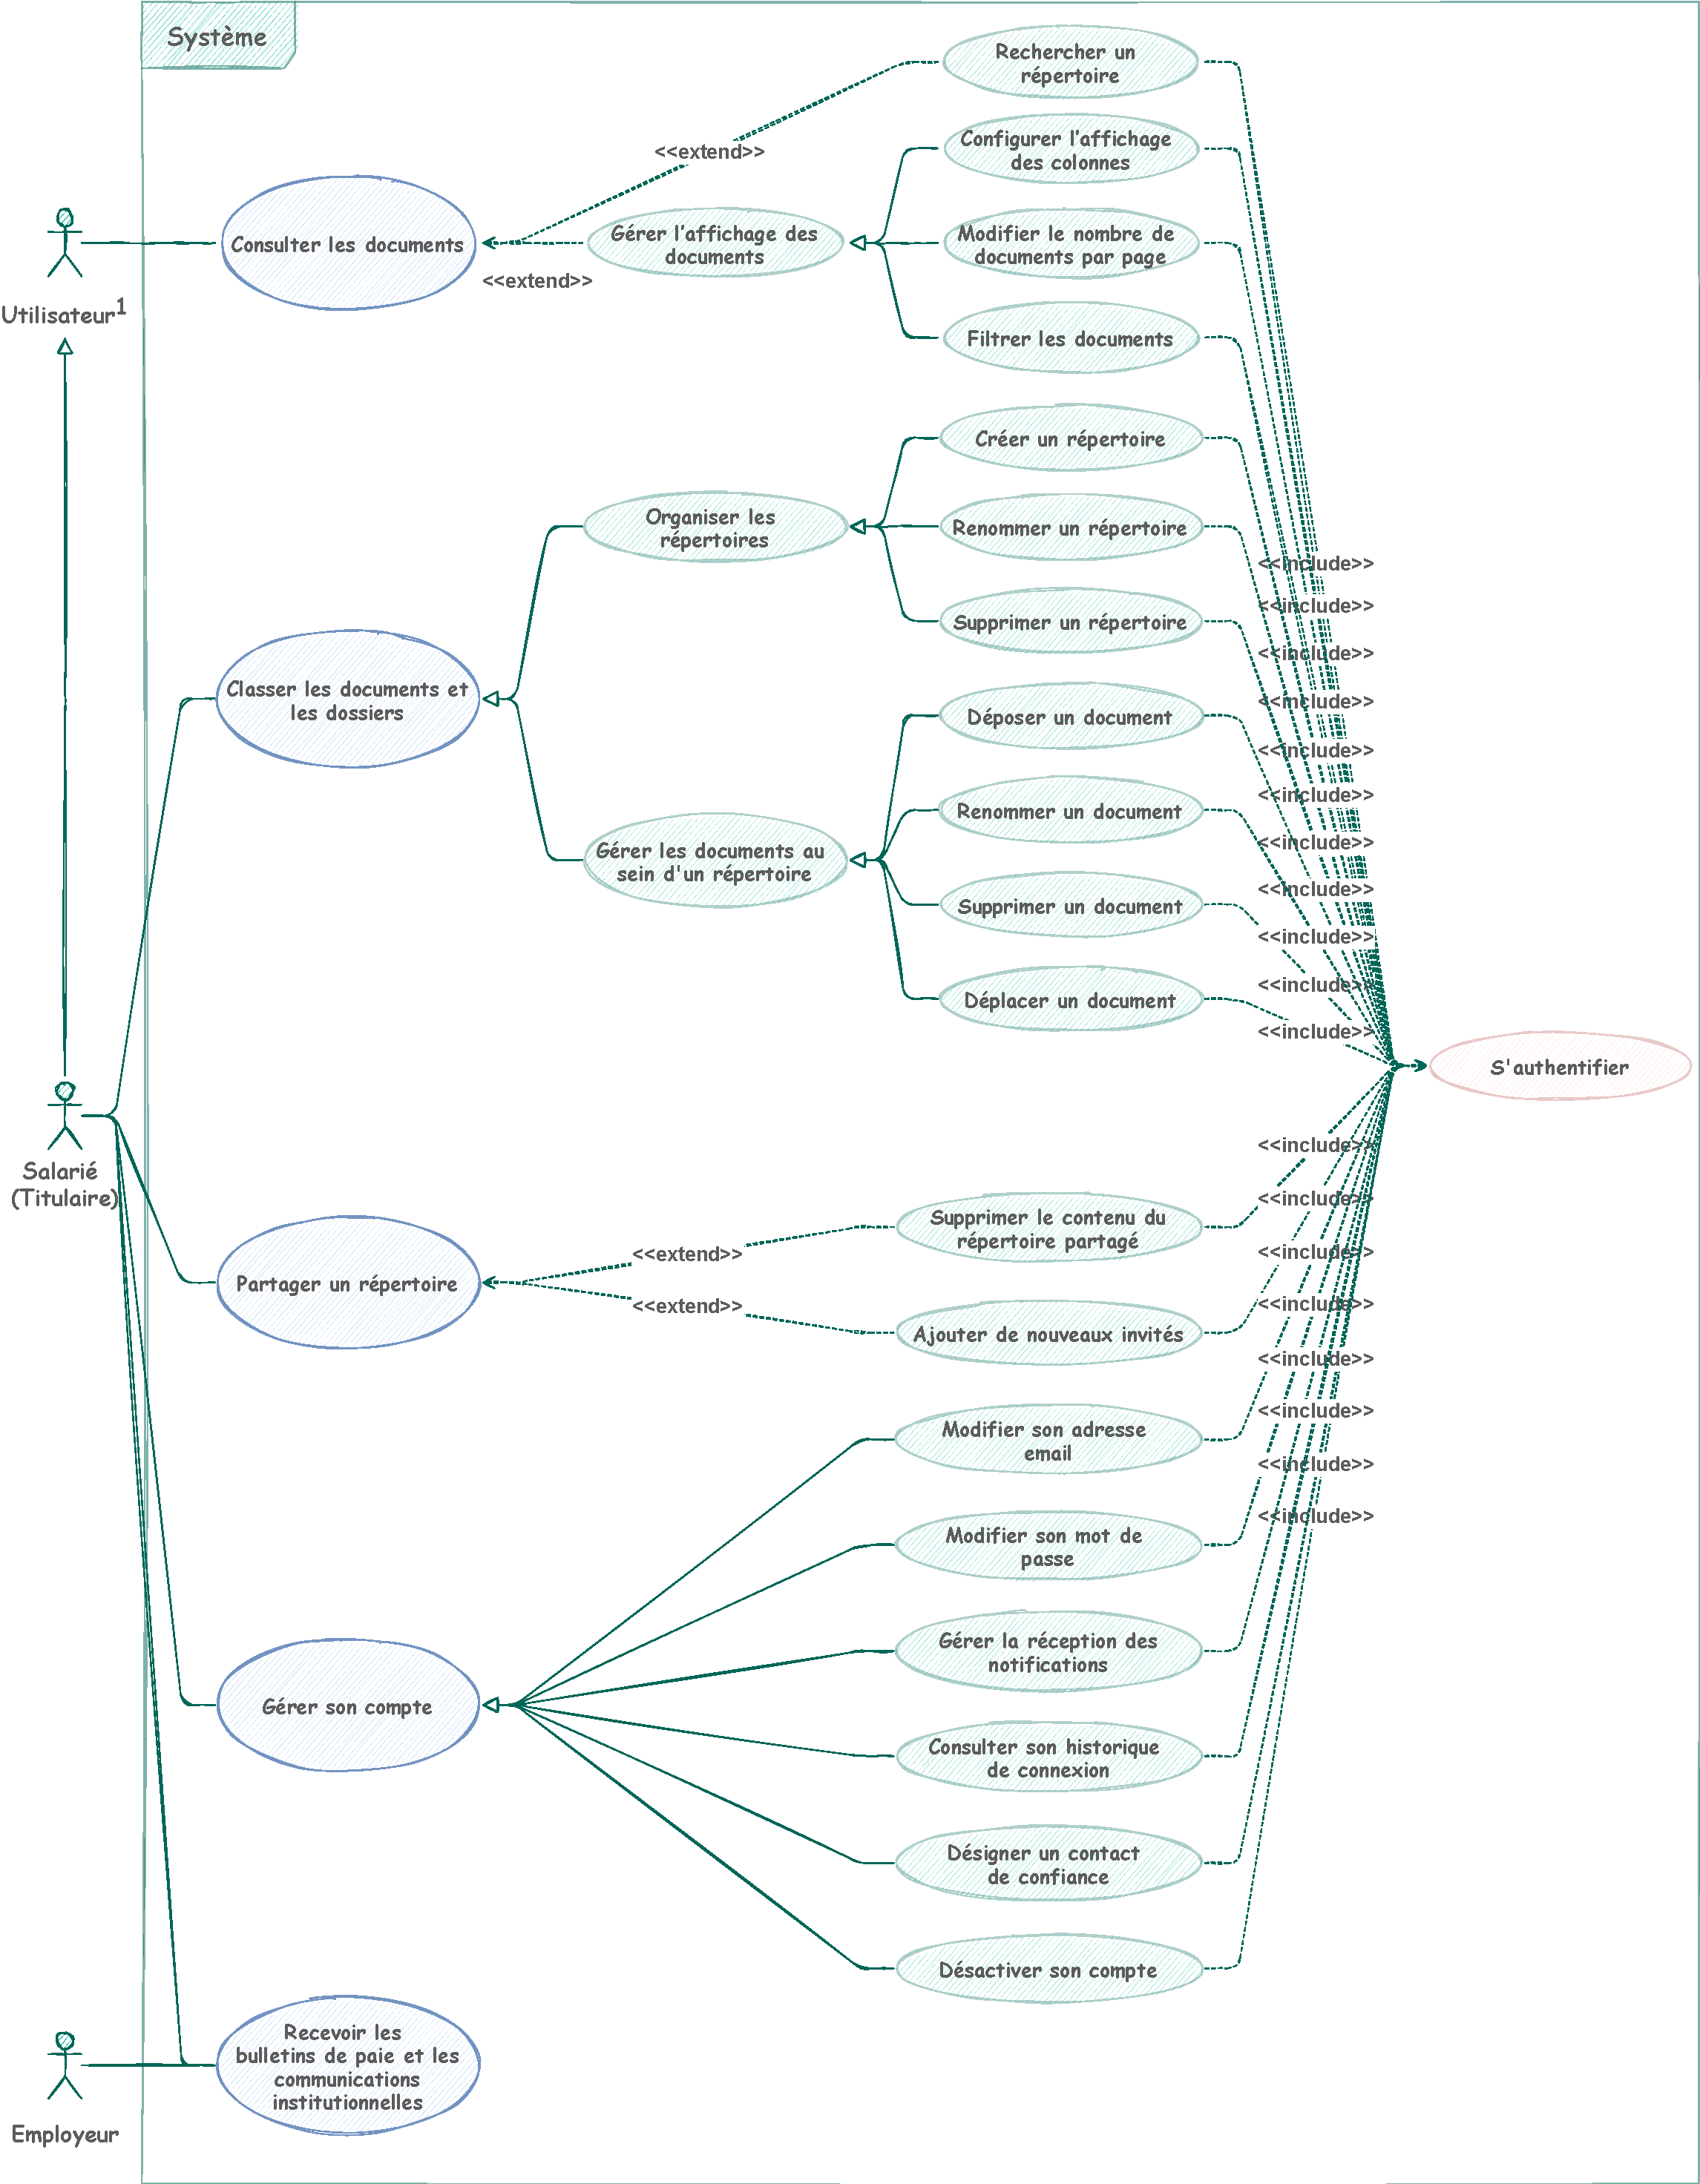
\includegraphics[width=1.1\linewidth]{images/sec3/usecase.pdf}
    \caption{Diagramme de cas d'utilisation général}
    \label{fig:uc}
\end{figure}
\footnotetext[1]{représente le cas d'un acteur (non propriétaire) autorisé à utiliser le compte.}
\hfill
\vspace{-1.5cm}
\subsubsection{Raffinement des cas d'utilisation prioritaires}
\subsubsubsection*{Cas d’utilisation : « S'inscrire »}
\setlength{\fboxrule}{1pt}
\setlength{\fboxsep}{6pt}
\begin{longtblr}[caption={Description textuelle du CU « S'inscrire »},
    note{1} = {Le mot de passe doit comporter un minimum de 8 caractères et un maximum de 20 caractères, au moins une lettre, au moins un chiffre, au moins un caractère spécial parmi @\#\$\%\^\&+=?\_|!,;.:\/ et ne doit pas contenir d'espaces.}]{
    hlines = {0.5pt,chambray},
    vlines = {0.5pt,chambray},
    colsep=4pt,
    rowsep=4pt,
    colspec={Q[l]X[l]},
    rowspec={Q[m] Q[m] Q[m] Q[m] Q[m] Q[m]},
}
\textbf{Acteur} & Salarié (Titulaire) \\
\textbf{Objectif}& 
L'inscription permet aux salariés d'activer la mise à disposition de leurs bulletins de paie électroniques dans leurs coffres-forts.\\
\textbf{Pré-condition} & 
Disposer d'une connexion Internet et d'un navigateur.\\
\textbf{Scénario} & 
\begin{minipage}{\linewidth}
\raggedright
\begin{enumerate}[leftmargin=*]
    \item Le salarié se rend sur \url{www.myarkevia.com} à l'aide d'un navigateur.
    \item Le salarié clique sur \fcolorbox{arkevia-btn-border}{arkevia-btn-bg}{\textcolor{white}{\scriptsize\textbf{JE M'INSCRIS}}}.
    \item Le salarié renseigne le matricule et le code secret qui lui ont été communiqués par le service RH, soit par des courriers spécifiques, soit par son dernier bulletin de salaire papier.
    \item Le salarié doit tenir compte de la \textbf{convention de mise à disposition du bulletin de paie électronique par l’employeur} et cocher la case \textcolor{gray}{\faCheckSquare\ J’ai lu et j’accepte les conditions de la convention} pour pouvoir passer à l’étape suivante.
    \item Le salarié renseigne les champs obligatoires concernant son profil.
   \item Le salarié doit tenir compte des \textbf{Conditions Générales d’Utilisation} et cocher la  case \textcolor{gray}{\faCheckSquare\ J’accepte les conditions générales d’utilisation d’ARKEVIA} pour pouvoir passer à l’étape suivante.
   \item Le salarié saisit son mot de passe conformément aux règles de sécurité\TblrNote{1}, puis le confirme.
   \item Enfin, le salarié clique sur \fcolorbox{arkevia-btn-border}{arkevia-btn-bg}{\textcolor{white}{\scriptsize\textbf{VALIDER MON INSCRIPTION}}} pour confirmer son inscription.
\end{enumerate}
\end{minipage}
\\
\textbf{Exception} & \begin{minipage}{\linewidth}
\raggedright
\begin{itemize}[leftmargin=*]
    \item Ouvert aux seuls salariés des entreprises ayant conclues un contrat de services avec CEGEDIM SRH (« Service ARKEVIA »)
    \item Le salarié saisit un matricule ou un code secret invalide.
    \item Le salarié saisit un mot de passe non conforme aux règles de sécurité définies par le système.
\end{itemize}
\end{minipage}
\\
\textbf{Post-condition} & Le système redirige automatiquement le salarié vers la page de connexion.\\
\end{longtblr}
\hfill
\vspace{-1.4cm}
\subsubsubsection*{Cas d’utilisation : « Se connecter »}
\begin{longtblr}[caption={Description textuelle du CU « Se connecter »}]{
    hlines = {0.5pt,chambray},
    vlines = {0.5pt,chambray},
    colsep=4pt,
    rowsep=4pt,
    colspec={Q[l]X[l]},
    rowspec={Q[m] Q[m] Q[m] Q[m] Q[m] Q[m]},
}
\textbf{Acteur} & Salarié, actuel ou passé, ayant ouvert et utilisant le coffre-fort électronique, et le cas échéant, les personnes physiques spécifiquement habilitées par le titulaire. \\
\textbf{Pré-condition} & 
\begin{minipage}{\linewidth}
\raggedright
\begin{itemize}[leftmargin=*]
    \item Avoir préalablement suivi la procédure d'inscription.
    \item Disposer d'une connexion Internet et d'un navigateur.
\end{itemize}
\end{minipage}
\\
\textbf{Scénario} & 
\begin{minipage}{\linewidth}
\raggedright
\begin{enumerate}[leftmargin=*]
    \item L'utilisateur se rend sur \url{www.myarkevia.com} à l'aide d'un navigateur.
    \item L'utilisateur saisit son adresse e-mail et son mot de passe.
    \begin{itemize}
        \item Si nécessaire, il peut cliquer sur l’oeil \faEye{ } dans le champ \textbf{Mot de passe} pour voir son mot de passe en toutes lettres et ainsi éviter des erreurs de saisie.
    \end{itemize}
   \item Le salarié clique sur \fcolorbox{arkevia-btn-border}{arkevia-btn-bg}{\textcolor{white}{\scriptsize\textbf{JE ME CONNECTE}}} pour confirmer son inscription.
\end{enumerate}
\end{minipage}
\\
\textbf{Exception} & \begin{minipage}{\linewidth}
\raggedright
\begin{itemize}[leftmargin=*]
    \item Le salarié entre un mot de passe ou un e-mail incorrect.
    \item Au-delà de trois tentatives erronées, le système suspecte un abus ou une utilisation illégale de la part de l'utilisateur et bloque donc l'accès au compte pour une période de 15 minutes.
\end{itemize}
\end{minipage}
\\
\textbf{Post-condition} & Le système redirige l'utilisateur vers la page d'accueil de son compte.\\
\end{longtblr}

\subsubsubsection*{Cas d’utilisation : « Créer un nouveau répertoire »}
\begin{longtblr}[caption={Description textuelle du CU « Créer un nouveau répertoire »}, note{2} = {Les noms de répertoire ne peuvent pas contenir d'espaces, ni de caractères non conformes aux règles de nommage des fichiers Unix.}]{
    hlines = {0.5pt,chambray},
    vlines = {0.5pt,chambray},
    colsep=4pt,
    rowsep=4pt,
    colspec={Q[l]X[l]},
    rowspec={Q[m] Q[m] Q[m] Q[m] Q[m] Q[m]},
}
\textbf{Acteur} & Salarié (Titulaire) \\
\textbf{Objectif}& 
Permettre au salarié de créer ses propres répertoires afin de stocker et classer ses documents (bulletins de paie ou documents personnels qu'il a déposés dans son coffre-fort).\\
\textbf{Pré-condition} & 
S'authentifier avec un identifiant correct.\\
\textbf{Scénario} & 
\begin{minipage}{\linewidth}
\raggedright
\begin{enumerate}[leftmargin=*]
    \item Dans la section répertoire de l'écran, le salarié sélectionne le dossier sous lequel il souhaite créer un répertoire. Le dossier sélectionné est alors marqué en vert.
    \item Le salarié clique sur l’icône \faPlusSquareO { }\textbf{Créer un nouveau répertoire}.
    \item Le salarié renseigne le nom du nouveau répertoire.
   \item Le salarié clique sur \fcolorbox{arkevia-btn-bg}{arkevia-btn-bg}{\textcolor{white}{\scriptsize\textbf{Créer}}}.
\end{enumerate}
\end{minipage}
\\
\textbf{Exception} & \begin{minipage}{\linewidth}
\raggedright
\begin{itemize}[leftmargin=*]
    \item Le nom du répertoire est invalide\TblrNote{2}.
    \item Création d'un répertoire avec un nom qui existe déjà.
\end{itemize}
\end{minipage}
\\
\textbf{Post-condition} & Le système renvoie un message indiquant à l'utilisateur qu'il peut désormais déposer des fichiers dans son nouveau répertoire.\\
\end{longtblr}


\subsubsubsection*{Cas d’utilisation : « Déposer un document »}
\begin{longtblr}[caption={Description textuelle du CU « Déposer un document »}]{
    hlines = {0.5pt,chambray},
    vlines = {0.5pt,chambray},
    colsep=4pt,
    rowsep=4pt,
    colspec={Q[l]X[l]},
    rowspec={Q[m] Q[m] Q[m] Q[m] Q[m] Q[m]},
}
\textbf{Acteur} & Salarié (Titulaire) \\
\textbf{Objectif}& 
Permettre aux salariés d'importer leurs documents importants.\\
\textbf{Pré-condition} & 
S'authentifier avec un identifiant correct.\\
\textbf{Scénario} & 
\begin{minipage}{\linewidth}
\raggedright
\begin{enumerate}[leftmargin=*]
    \item Le salarié sélectionne un dossier sous lequel il souhaite importer ses documents.
    \item Le salarié clique sur \fcolorbox{white}{arkevia-btn-bg2}{\textcolor{white}{ \scriptsize\textbf{\faFileO { } Déposer un document}}}.
   \item Dans la fenêtre \textbf{Ajout d’un document}, le salarié clique sur \fcolorbox{gray6}{gray!20!white}{\scriptsize\textbf{Choisir un fichier}}.
   \item Le salarié parcourt ses répertoires et sélectionne un fichier. Il peut éventuellement sélectionner plusieurs fichiers en appuyant sur la touche Ctrl et en cliquant simultanément avec la souris sur les fichiers souhaités.
    \item Le salarié clique sur \fcolorbox{arkevia-btn-bg}{arkevia-btn-bg}{\textcolor{white}{\scriptsize\textbf{Ajouter}}}.
\end{enumerate}
\end{minipage}
\\
\textbf{Exception} & 
Le fichier dépasse la taille limite autorisée de 50 Mo.\\
\textbf{Post-condition} & Le système renvoie un message indiquant à l'utilisateur que les documents sont en cours d'importation, puis un autre message indiquant le statut de l'opération lorsqu'elle est terminée.
\end{longtblr}

\subsubsubsection*{Cas d’utilisation : « Gérer un document »}
\begin{longtblr}[caption={Description textuelle du CU « Gérer un document »}]{
    hlines = {0.5pt,chambray},
    vlines = {0.5pt,chambray},
    colsep=4pt,
    rowsep=4pt,
    colspec={Q[l]X[l]},
    rowspec={Q[m] Q[m] Q[m] Q[m] Q[m] Q[m]},
}
\textbf{Acteur} & Salarié (Titulaire) \\
\textbf{Objectif}& 
Permettre aux salariés d'importer leurs documents importants.\\
\textbf{Pré-condition} & 
S'authentifier avec un identifiant correct.\\
\textbf{Scénario} & 
\begin{minipage}{\linewidth}
\raggedright
\begin{enumerate}[leftmargin=*]
    \item Le salarié sélectionne un répertoire pour accéder à son contenu.
    \item Dans la partie \textbf{Détail du répertoire} de l’écran, Il peut cliquer sur :
    \begin{itemize}
        \item L’icône \textcolor{gray7}{\textbf{Consulter} \faEye{ }} pour consulter le document.
        \item L’icône \textcolor{gray7}{\textbf{Renommer} \faPencil{ }} pour renommer le document.
        \item L’icône \textcolor{gray7}{\textbf{Supprimer} \faTrash{ }} pour supprimer le document.
        \item Le \textbf{nom du document} et, tout en maintenant le clic, il peut le glisser-déposer dans un répertoire de son choix.
    \end{itemize}
\end{enumerate}
\end{minipage}
\\
\textbf{Exception} & 
\begin{minipage}{\linewidth}
\raggedright
\begin{itemize}[leftmargin=*]
    \item Les documents professionnels déposés par l'employeur ne peuvent pas être supprimés par le salarié.
    \item Le nom du document ne peut pas être renommé avec un nom qui existe déjà dans le répertoire parent.
\end{itemize}
\end{minipage}
\\
\textbf{Post-condition} & 
Pour chaque action effectuée, le système renvoie un message indiquant à l'utilisateur l'état de l'opération lorsqu'elle est terminée.//
\end{longtblr}

\subsubsubsection*{Cas d’utilisation : « Gérer l'affichage des documents »}
\begin{longtblr}[caption={Description textuelle du CU « Gérer l'affichage des documents »}, , note{3} = {Les filtres actifs s’affichent au-dessus de la section \textbf{Détail du répertoire}.}]{
    hlines = {0.5pt,chambray},
    vlines = {0.5pt,chambray},    
    colsep=4pt,
    rowsep=4pt,
    colspec={Q[l]X[l]},
    rowspec={Q[m] Q[m] Q[m] Q[m] Q[m] Q[m]},
}
\textbf{Acteur} & Salarié (Titulaire) \\
\textbf{Objectif}& 
Permettre aux salariés de configurer l’affichage des colonnes du tableau \textbf{Détail du répertoire}, de filtrer les  documents ainsi que d'ajuster le nombre de documents affichés par page.
\\
\textbf{Pré-condition} & 
S'authentifier avec un identifiant correct.\\
\textbf{Scénario} & 
\begin{minipage}{\linewidth}
\raggedright
\begin{itemize}[leftmargin=*]
    \item Pour configurer l’affichage des colonnes : 
    \begin{enumerate}
        \item Le salarié sélectionne un répertoire pour en afficher le contenu dans le tableau \textbf{Détail du répertoire}.
        \item Le salarié clique sur la liste déroulante \textbf{Gérer les colonnes} et coche les colonnes qu'il souhaite afficher et décoche celles qu'il souhaite masquer.
    \end{enumerate}
    \item Si le répertoire contient un grand nombre de documents, ils sont alors affichés sur plusieurs pages que le salarié peut parcourir à l'aide des boutons situés sous le tableau. Pour plus de commodité, le salarié a la possibilité d'afficher plus de lignes dans le tableau et ainsi de réduire le nombre de pages. Pour ce faire :
    \begin{enumerate}
        \item Le salarié clique sur la liste déroulante \textbf{[X] lignes}.
        \item Le salarié sélectionne 5, 10 ou 20 lignes.
    \end{enumerate}
    \item Le salarié a également la possibilité de filtrer les documents pour n'afficher que ceux correspondant aux critères de sélection qu'il a choisis. Pour ce faire :
    \begin{enumerate}
        \item Le salarié clique sur le bouton \fcolorbox{arkevia-btn-bg}{arkevia-btn-bg}{\textcolor{white}{\scriptsize\textbf{Filtrer } \faSliders}}.
        \item Parmi les 5 filtres proposés, le salarié clique sur les filtres souhaités. 
        \item Dans le champ qui s’affiche, le salarié renseigne les critères de filtrage.
        \item Le salarié clique  sur \fcolorbox{arkevia-btn-bg}{arkevia-btn-bg}{\textcolor{white}{\scriptsize\textbf{Appliquer les filtres}}}\TblrNote{3}.
        \item Le salarié clique sur la croix \textcolor{gray}{\faClose} pour fermer le volet des filtres.
    \end{enumerate}
    \item Pour désactiver le filtrage :
    \begin{enumerate}
        \item Le salarié clique sur le bouton \fcolorbox{arkevia-btn-bg}{arkevia-btn-bg}{\textcolor{white}{\scriptsize\textbf{Filtrer } \faSliders}} pour afficher le volet des filtres.
        \item Pour désactiver tous les filtres, le salarié clique sur le bouton Annuler \fcolorbox{arkevia-btn-bg}{white}{\textcolor{gray}{\faRefresh}}.
        \item Le salarié peut également désactiver certains filtres en cliquant sur le filtre à désactiver puis sur la croix \fcolorbox{white}{arkevia-btn-bg}{\textcolor{white}{\faClose}} pour supprimer les critères saisis.
A la fin, l'employé clique sur Appliquer les filtres pour rafraîchir la liste des documents.
\item Le salarié clique sur la croix \textcolor{gray}{\faClose} pour fermer le volet des filtres.
    \end{enumerate}
\end{itemize}
\end{minipage}
\\
\textbf{Exception} & Aucune
\\
\textbf{Post-condition} & 
Pour chaque action effectuée, l’affichage est instantanément modifié.
\end{longtblr}
\break
\subsubsubsection*{Cas d’utilisation : « Gérer le partage des documents »}
\begin{longtblr}[caption={Description textuelle du CU « Partager un répertoire »},
note{4} = {La date saisie doit être postérieure à la date du jour.},
note{5} = {En ajoutant des documents au dossier  partagé, l'utilisateur crée simplement une copie des documents d'origine. Ils ne sont en aucun cas supprimés du répertoire d’origine.},
note{6} = {Il est impératif de cocher la case Envoyer une notification aux invités, sinon ils ne recevront pas de notification pour télécharger les documents qui leur sont partagés.}]{
    hlines = {0.5pt,chambray},
    vlines = {0.5pt,chambray},   
    colsep=4pt,
    rowsep=4pt,
    colspec={Q[l]X[l]},
    rowspec={Q[m] Q[m] Q[m] Q[m] Q[m] Q[m]},
}
\textbf{Acteur} & Salarié (Titulaire) \\
\textbf{Objectif}& 
Donnez aux salariés la possibilité de créer des répertoires de partage afin qu'ils puissent partager des documents avec des tiers en dehors de leur entreprise.\\
\textbf{Pré-condition} & 
S'authentifier avec un identifiant correct.\\
\textbf{Scénario} & 
\begin{minipage}{\linewidth}
\raggedright
\begin{enumerate}[leftmargin=*]
    \item Le salarié doit d'abord créer un répertoire partagé, cela peut être fait à travers le scénario suivant :
    \begin{enumerate}
        \item Dans la liste des répertoires, le salarié clique sur le dossier \textbf{Partage}.
        \item Le salarié clique sur l’icône \textbf{Ajouter un répertoire partagé} \faShareAltSquare.
        \item Dans la fenêtre \textbf{Nouveau partage}, le salarié renseigne les champs suivants :
        \begin{itemize}
            \item \textbf{Nom du répertoire}.
            \item \textbf{Liste des invités} : il saisit les adresses e-mail des personnes avec lesquelles il souhaite partager ses documents, séparées par une virgule.
            \item \textbf{Commentaire}.
            \item \textbf{Date d’expiration du partage} : il saisit la date\TblrNote{4} jusqu’à laquelle le tiers pourra accéder au contenu de son répertoire de partage.
        \end{itemize}
        \item Le salarié clique sur \fcolorbox{arkevia-btn-bg}{arkevia-btn-bg}{\textcolor{white}{\scriptsize\textbf{Créer}}}.
    \end{enumerate}
    \item Pour ajouter des documents dans le répertoire partagé, le salarié sélectionne et glisse les documents vers le répertoire partagé précédemment créé\TblrNote{5}.
    \item Le salarié clique sur l’icône \textbf{Invitation partage} {\hspace{2pt}}\faFileTextO {\hspace{-13pt}\footnotesize\faInfoCircle}{\hspace{6pt}.}
    \item Éventuellement, le salarié peut :
    \begin{itemize}
        \item Ajouter de nouveaux e-mails d'invités dans le champ \textbf{Liste d’invités}.
        \item Modifiez la date d’expiration du partage.
    \end{itemize}
    \item Le salarié coche la case \textbf{Envoyer une notification aux invités}\TblrNote{6}.
    \item Le salarié clique sur \fcolorbox{arkevia-btn-bg}{arkevia-btn-bg}{\textcolor{white}{\scriptsize\textbf{Mettre à jour}}}.
\end{enumerate}
\end{minipage}
\\
\textbf{Exception} & 
    L'utilisateur inscrit un e-mail dont le format est considéré comme invalide.\\
\textbf{Post-condition} & 
Les invités reçoivent un mail contenant un lien de téléchargement des documents partagés qui sera actif jusqu’à la date d’expiration du partage. Une fois la date d’expiration atteinte, le répertoire partagé est supprimé du dossier \textbf{Partage}.
\end{longtblr}


\begin{longtblr}[caption={Description textuelle du CU « Supprimer un partage »}, note{7} = {Pour supprimer tous les documents du dossier partagé, le salarié doit supprimer individuellement chaque document contenu au sein du répertoire.}]{
    hlines = {0.5pt,chambray},
    vlines = {0.5pt,chambray}, 
    colsep=4pt,
    rowsep=4pt,
    colspec={Q[l]X[l]},
    rowspec={Q[m] Q[m] Q[m] Q[m] Q[m] Q[m]},
}
\textbf{Acteur} & Salarié (Titulaire) \\
\textbf{Objectif}& 
Supprimer tout ou partie des documents partagés avec un tiers avant la date d'expiration du partage.\\
\textbf{Pré-condition} & 
S'authentifier avec un identifiant correct.\\
\textbf{Scénario} & 
\begin{minipage}{\linewidth}
\raggedright
\begin{enumerate}[leftmargin=*]
    \item Le salarié sélectionne le dossier partagé dans le dossier \textbf{Partage}.
    \item Dans la section \textbf{Détail du répertoire}, le salarié clique sur l’icône \textcolor{gray7}{\textbf{Supprimer} \faTrash{ }} pour supprimer le document du répertoire\TblrNote{7}.
\end{enumerate}
\end{minipage}
\\
\textbf{Exception} & Aucune.\\
\textbf{Post-condition} & 
Le répertoire partagé restera visible dans la liste des répertoires partagés jusqu'à ce que la date d'expiration du partage soit atteinte. Si les invités cliquent sur le lien de téléchargement, le répertoire téléchargé ne contiendra pas les documents supprimés ou sera vide si le salarié a choisi de supprimer tous les documents.
\end{longtblr}


\subsubsubsection*{Gestion de compte}
Pour accéder à la gestion de son compte, le salarié clique sur l’icône \textbf{Mon compte}. Plusieurs fonctionnalités sont proposées :

\begin{longtblr}[caption={Description textuelle du CU « Modifier son adresse email »}]{
    hlines = {0.5pt,chambray},
    vlines = {0.5pt,chambray},
    colsep=4pt,
    rowsep=4pt,
    colspec={Q[l]X[l]},
    rowspec={Q[m] Q[m] Q[m] Q[m] Q[m] Q[m]},
}
\textbf{Acteur} & Salarié (Titulaire) \\
\textbf{Objectif} & 
L'adresse e-mail est utilisée comme login pour le coffre-fort d'Arkevia. C'est également l'adresse où l'acteur reçoit les notifications lorsqu'un document est déposé dans son coffre-fort.\\
\textbf{Pré-condition} & 
S'authentifier avec un identifiant correct.\\
\textbf{Scénario} & 
\begin{minipage}{\linewidth}
\raggedright
\begin{enumerate}[leftmargin=*]
    \item Le salarié clique sur l’onglet \textbf{Mes informations personnelles}.
    \item Ensuite, il remplit la nouvelle adresse dans le champ \textbf{E-mail}, puis la confirme dans le champ \textbf{Confirmer E-mail*}.
    \item Enfin, le salarié clique sur 
    \fcolorbox{arkevia-btn-bg}{arkevia-btn-bg}{\textcolor{white}{\scriptsize\textbf{MODIFIER}}}.
\end{enumerate}
\end{minipage}
\\
\textbf{Exception} & \begin{minipage}{\linewidth}
\raggedright
\begin{itemize}[leftmargin=*]
    \item L'employé introduit une adresse électronique qui ne suit pas les règles du format email standard.
    \item Les deux champs \textbf{E-mail} et \textbf{Confirmer E-mail*} ne sont pas identiques.
\end{itemize}
\end{minipage}
\\
\textbf{Post-condition} & La nouvelle adresse électronique devient alors le nouveau identifiant du salarié.
\\
\end{longtblr}

\begin{longtblr}[caption={Description textuelle du CU « Modifier son mot de passe »}, note{8}={Le nouveau mot de passe doit respecter les règles de sécurité listées dans
    la partie droite de l’écran}]{
    hlines = {0.5pt,chambray},
    vlines = {0.5pt,chambray},  
    colsep=4pt,
    rowsep=4pt,
    colspec={Q[l]X[l]},
    rowspec={Q[m] Q[m] Q[m] Q[m] Q[m] Q[m]},
}
\textbf{Acteur} & Salarié (Titulaire) \\
\textbf{Objectif} & 
La politique de sécurité impose un changement de mot de passe tous les deux mois. Dès que le délai est expiré, il sera nécessaire de le changer lors de la connexion au coffre-fort. Cependant, il est possible de le changer librement à tout moment.\\
\textbf{Pré-condition} & 
S'authentifier avec un identifiant correct.\\
\textbf{Scénario} & 
\begin{minipage}{\linewidth}
\raggedright
\begin{enumerate}[leftmargin=*]
    \item Le salarié clique sur l’onglet \textbf{Mon mot de passe}.
    \item Le salarié saisit son mot de passe actuel.
    \item Ensuite, il saisit son nouveau mot de passe\TblrNote{8}, puis le confirme.
    \item Enfin, le salarié clique sur 
    \fcolorbox{arkevia-btn-bg}{arkevia-btn-bg}{\textcolor{white}{\scriptsize\textbf{MODIFIER}}}.
\end{enumerate}
\end{minipage}
\\
\textbf{Exception} & Le salarié saisit un mot de passe non conforme aux règles de sécurité définies par le système.
\\
\textbf{Post-condition} & L'ancien mot de passe est changé.
\\
\end{longtblr}

\begin{longtblr}[caption={Description textuelle du CU « Consulter son historique de connexion »}]{
    hlines = {0.5pt,chambray},
    vlines = {0.5pt,chambray},
    colsep=4pt,
    rowsep=4pt,
    colspec={Q[l]X[l]},
    rowspec={Q[m] Q[m] Q[m] Q[m] Q[m] Q[m]},
}
\textbf{Acteur} & Salarié (Titulaire) \\
\textbf{Objectif} & 
Chaque connexion au coffre-fort est historisée. Le salarié peut recevoir une notification par email à chaque connexion et ainsi être averti de tout accès involontaire à son coffre-fort.\\
\textbf{Pré-condition} & 
S'authentifier avec un identifiant correct.\\
\textbf{Scénario} & 
\begin{minipage}{\linewidth}
\raggedright
\begin{enumerate}[leftmargin=*]
    \item Le salarié clique sur l’onglet \textbf{Historique de connexion}.
    \item Le salarié peut cliquer sur \fcolorbox{white}{olive4}{\textcolor{white}{\scriptsize \faFileExcelO{ } \textbf{Exporter en Excel}}}  ou \fcolorbox{white}{red6}{\textcolor{white}{\scriptsize \faFilePdfO{ }  \textbf{Exporter en PDF}}} pour récupérer la liste complète des connexions à son coffre-fort.
    \item Le salarié peut également cocher/décocher la case \textcolor{gray}{\faCheckSquare\ Être averti par e-mail des connexions sur mon compte} pour recevoir ou non une notification à chaque fois que son compte est ouvert, puis cliquer sur  
    \fcolorbox{arkevia-btn-bg}{arkevia-btn-bg}{\textcolor{white}{\scriptsize\textbf{MISE À JOUR}}} pour enregistrer la modification.
\end{enumerate}
\end{minipage}
\\
\textbf{Exception} & Aucune.
\\
\textbf{Post-condition} & Un tableau affiche les six dernières connexions (date et heure de connexion ainsi
que l’adresse IP à partir de laquelle a eu lieu la connexion).
\\
\end{longtblr}

\begin{longtblr}[caption={Description textuelle du CU « Désigner un contact de confiance »}]{
    hlines = {0.5pt,chambray},
    vlines = {0.5pt,chambray},
    colsep=4pt,
    rowsep=4pt,
    colspec={Q[l]X[l]},
    rowspec={Q[m] Q[m] Q[m] Q[m] Q[m] Q[m]},
}
\textbf{Acteur} & Salarié (Titulaire) \\
\textbf{Objectif} & 
Pouvoir désigner une personne de confiance qui pourra récupérer le contenu du coffre-fort du salarié si ce dernier n'est plus en mesure de l'utiliser.\\
\textbf{Pré-condition} & 
S'authentifier avec un identifiant correct.\\
\textbf{Scénario} & 
\begin{minipage}{\linewidth}
\raggedright
\begin{enumerate}[leftmargin=*]
    \item Le salarié clique sur l’onglet \textbf{ Contact de confiance}.
    \item Le salarié remplit le formulaire avec l’identité de la personne de confiance.
    \item Il confirme son choix en cochant la case autorisant le contact à accéder au contenu de son coffre-fort.
    \item Enfin, il clique sur  
    \fcolorbox{arkevia-btn-bg}{arkevia-btn-bg}{\textcolor{white}{\scriptsize\textbf{VALIDER}}} pour enregistrer cette modification.
\end{enumerate}
\end{minipage}
\\
\textbf{Exception} & Aucune.
\\
\textbf{Post-condition} & Le contact de confiance est désigné.
\\
\end{longtblr}

\begin{longtblr}[caption={Description textuelle du CU « Désactiver son compte »}]{
    hlines = {0.5pt,chambray},
    vlines = {0.5pt,chambray},
    colsep=4pt,
    rowsep=4pt,
    colspec={Q[l]X[l]},
    rowspec={Q[m] Q[m] Q[m] Q[m] Q[m] Q[m]},
}
\textbf{Acteur} & Salarié (Titulaire) \\
\textbf{Objectif} & 
Demander la désactivation du compte ARKEVIA. \\
\textbf{Pré-condition} & 
S'authentifier avec un identifiant correct.\\
\textbf{Scénario} & 
\begin{minipage}{\linewidth}
\raggedright
\begin{enumerate}[leftmargin=*]
    \item Le salarié clique sur l’onglet \textbf{ Désactivation du compte}.
    \item Le salarié tenir compte et lire attentivement les informations relatives à la désactivation de son compte.
    \item Le salarié coche la case \textcolor{gray}{\faCheckSquare{ } Désactivation du compte ARKEVIA}
    \item Enfin, il clique sur  
    \fcolorbox{arkevia-btn-bg}{arkevia-btn-bg}{\textcolor{white}{\scriptsize\textbf{ACCEPTER}}}.
\end{enumerate}
\end{minipage}
\\
\textbf{Exception} & Si le salarié a une inscription activée aux bulletins de paie électroniques auprès de son employeur, il doit au préalable se désinscrire auprès de son service RH. Sans cette désinscription avant désactivation du compte, l'employeur continuera d’y déposer ses bulletins de paie électroniques sans que lui puisse y accéder.
\\
\textbf{Post-condition} & Le salarié recevra un lien par email, actif pendant une heure, pour confirmer la désactivation de son compte.
\\
\end{longtblr}
\subsection{Analyse des besoins}
\subsubsection{Migration du socle technique}
La migration du socle technique consiste à faire évoluer le stack applicatif d'un projet, pour évoluer généralement sur une technologie plus récente. Une telle migration de projet applicatif englobe un certain nombre de variables qu'il convient maîtriser (migration de données, de technologies, de fichiers...), ce dernier peut vite devenir complexe.\\


Il y a deux principaux cas qui conduisent à entamer un projet de migration :
\begin{itemize}
    \item \textbf{La migration de projet contrainte par les éditeurs et l'évolution des briques applicatives (bases de données, frameworks, technologies...)}. Un projet applicatif est composé d'un ensemble de briques applicatives qui suivent chacune leur propre cycle, qui est souvent très rapide ! En effet, les éditeurs mettent régulièrement à jour leurs solutions, et très vite, les anciennes versions ne sont plus supportées (ce qui pose des problèmes en termes de sécurité, de maintenabilité et de compatibilité). Il est donc impératif de suivre de très près l'évolution des briques applicatives.
    \item \textbf{La migration volontaire de projet (plus rare)} : permet d'anticiper l'évolution du projet et/ou du SI, et de mieux préparer l'avenir sur des bases solides et récentes.\\
\end{itemize}

Dans ce contexte, j'ai dû entreprendre le sujet de la migration afin d'évoluer vers une solution plus optimale tout en préservant la cohérence globale du système en question. Ces migrations représentent un double défi : d'une part rattraper le retard technologique des anciennes briques du système et d'autre part s'assurer que l'application fonctionnera bien, et qu'elle ne sera pas confrontée à des limites de développement de nouvelles fonctionnalités.\\

Nul doute que tous ces défis s’accompagnent de réflexions globales sur le métier, les infrastructures, les applications et la culture pour assurer la cohérence totale des futurs processus créés. Dans cet opus, nous allons nous intéresser à une partie de ces chantiers qui est la migration du framework de base Spring.\\

Avant d'entamer un chantier de transformation d’une telle ampleur, la compréhension du besoin client est fondamentale pour une migration d’un bloc applicatif Legacy vers une nouvelle base. Pour clôturer cette section, nous allons identifier les principales étapes qui serviront à la réalisation de la migration au cours de ses différentes phases que nous allons détailler ci-dessous :\\ 

\begin{enumerate}
    \item La première phase est celle de l’audit et de la récolte d’information. Le but est de se familiariser avec le contexte global de la migration :
    \begin{enumerate}
        \item Audit global du périmètre SI à migrer ;
        \item Étude des documents d’architecture techniques et fonctionnels ;
        \item Déterminer les scores techniques des différentes briques applicatives : chaque brique applicative sera évaluée selon plusieurs critères. Parmi ces critères évalués, nous pouvons citer les suivants :
        \begin{itemize}
            \item La criticité de l’application ;
            \item Les technologies et Frameworks utilisés ;
            \item Les besoins métiers futurs (les évolutions des processus) ;
            \item Les prérequis de l’infrastructure cible ;
            \item Les transformations globales en cours de réalisation (Agilité, conteneurisation ou autre évolution technique, changement d’infrastructure en cours, etc.) ;
            \item L’estimation de l’effort de migration ;
            \item La conformité avec les standards de développement.
        \end{itemize}
        \item Revoir les contraintes techniques et opérationnelles ;
        \item Analyser les risques d’une manière plus détaillée pour chaque périmètre applicatif ;
        \item Évaluer les points de blocage.
    \end{enumerate}
    \item Au terme de la première phase, nous disposerons d'une vision détaillée du SI qui décrira précisément, via des spécifications techniques, les actions qui seront menées, les modalités de la stratégie de migration, et la trajectoire que l’on voudra lui donner à court, à moyen, ou à long terme, ce qui nous permettra au final de bien procéder aux travaux de développement de la migration.
\end{enumerate}
\subsubsection{Refactorisation et nettoyage du code}
\subsubsubsection{Refactorisation des modules applicatifs}
Arkevia est composée de huit modules permettant de gérer les différents aspects de l'application :
\begin{itemize}
    \item \textbf{HS-SY-Portal} :
    Ce module contient tous les éléments qui composent le corps du front-end Arkevia, y compris les composants Vue, les scripts, les images et les feuilles de style.
    \item \textbf{HS-SY-Client-Arkevia} :
    Ce module regroupe tous les services propres au client Arkevia, notamment l'inscription, la désactivation du compte, l'exportation de documents, etc.
    \item \textbf{HS-SY-Client-Standard} :
    Ce module comprend tous les services standards et les classes d'écran utilisés dans l'application.
    \item \textbf{HS-SY-Ged-Master} :
    Ce module comprend les services de gestion des répertoires et des documents, y compris la consommation de l'API SignArchive.
    \item \textbf{HS-SY-Master} : Ce module inclut les services de configuration, d'authentification, de gestion des comptes, etc.
    \item \textbf{HS-SY-Master-Domain} : Ce module permet de gérer les interactions avec la base de données, il rassemble toutes les entités qui sont utilisées pour faire le mapping avec les tables. On y trouve aussi tous les objets d'accès aux données.
    \item \textbf{HS-SY-Ged-Domain} : Ce module regroupe toutes les entités spécifiques à la gestion des documents, qui serviront à faire le mapping avec les tables.
    \item \textbf{HS-SY-Referentiel} : Ce module expose les services et les méthodes nécessaires pour établir la connexion avec l'API de SignArchive par le biais de requêtes Solr.\\
\end{itemize}

L'objectif est de réorganiser, restructurer et clarifier le code existant. Le besoin est de factoriser les modules clients pour rendre l'application plus générique. Pour ce faire, nous devons d'abord étudier la possibilité de virer le module \lstinline|HS-SY-Client-Standard|. Si cela est faisable, nous serons amenés à fédérer toute la partie gestion des écrans clients du module \lstinline|HS-SY-Client-Standard| au module \lstinline|HS-Sy-Client-Arkevia|, puis à retirer entièrement le module \lstinline|HS-SY-Client-Standard| du projet.\\

D'autre part, pour garder plus de clarté et d'organisation dans les fichiers de POM, nous pourrons également détacher les liens de dépendance directe entre les modules pour ne garder au final qu'un seul lien de dépendance transitif entre ces modules (voir figure \ref{fig:modules_arkevia}).
\begin{figure}[H]
    \begin{center}
        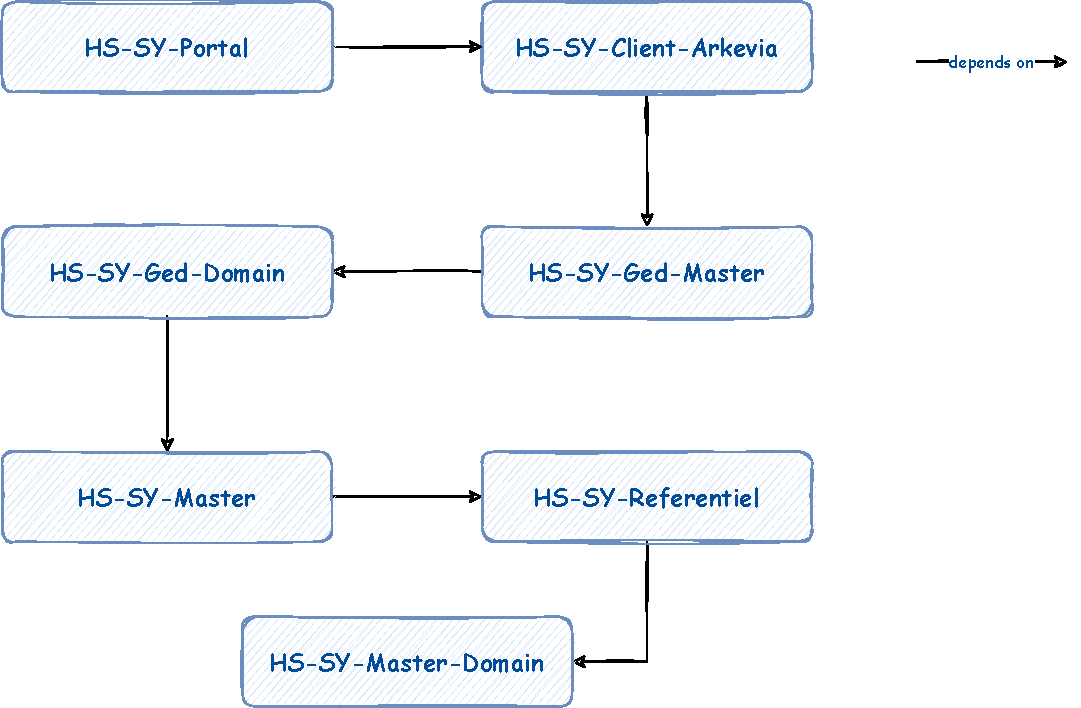
\includegraphics[width=0.6\linewidth]{images/sec4/dep.pdf}
        \caption{Architecture modulaire d'Arkevia}
        \label{fig:modules_arkevia}
    \end{center}
\end{figure}
\subsubsubsection{Renoncer à recourir à la brique de contrôle}
La brique de contrôle (Semantic Model And Business Control) est un service web tiers utilisé pour charger des métadonnées qui servent principalement d'en-tête pour le tableau de description des documents.\\
Suite à un audit mené sur l'application Arkevia afin d'identifier et de déboguer les réponses des appels provenant de cette brique, un total de douze appels a été relevé dans le code de l'application. En effet, cette brique de contrôle soulève des problèmes de performance, notamment un problème de temps d'arrêt très élevé. Afin d'éviter ce goulot d'étranglement, il a été convenu d'éliminer cette dépendance et de la remplacer par un simple appel à la base de données compte tenu que les réponses provenant de cette brique ne sont rien d'autre que des données et des configurations statiques.
\subsubsubsection{Retrait des dépendances inutilisables}
C'est un scénario typique, lorsque l'application est en cours de développement, et que plusieurs membres de l'équipe travaillent dessus, on risque de se trouver face à une série de dépendances inutiles dans les fichiers pom.xml du projet.\\
Il est alors ardu de déterminer manuellement quels sont les jars que l'application ne requiert pas. Pour résoudre ce problème, nous pouvons nous servir du plugin maven-dependency, en particulier l'objectif \lstinline|dependency:analyze|, qui permet d'analyser les dépendances du projet et de déterminer celles qui sont : utilisées et déclarées ; utilisées et non déclarées ; utilisées et déclarées.
\subsubsection{Optimisation du mécanisme d'envoi des notifications}
Le mécanisme de notification est responsable de prévenir un utilisateur par email lorsqu'il y a un nouveau dépôt de document (par exemple un bulletin de salaire) sur son coffre-fort par l'entreprise à laquelle il est abonné.\\

Prérequis nécessaire à la compréhension de sujet :
\begin{itemize}
    \item \textbf{Document} :  bulletins de paie, ou tout autre document RH au format dématérialisé.
    \item \textbf{Lot de documents} :  un nombre limité (batch) de documents (ajustables).
    \item \textbf{Notification} : Un mail générique transmis à un utilisateur pour le notifier du dépôt d'un document.
    \item \textbf{Scan} : une requête lancée à l'API SignArchive afin de vérifier s'il y a des dépôts de documents.
    \item \textbf{Cron} : une tâche planifiée qui déclenche l'exécution du Scan toutes les deux heures (configurable).
\end{itemize}
\subsubsubsection*{Récupération de données}
Le processus de notification est déclenché toutes les deux heures grâce à l'annotation \textbf{@Scheduled} fournie par Spring.\\
Tout d'abord, nous récupérons la date du dernier scan effectué, et nous enregistrons le nouveau scan avec la date du jour dans la table \lstinline|GED_BATCH_SCAN_UPLOAD_DOC|. Le date du dernier scan est utilisé par la suite, pour récupérer tous les documents déposés à partir de cette date jusqu'à le moment de lancement du nouveau scan.
\newpage
\begin{longtblr}[caption={Exemple de déroulement du Cron}]{
    hlines = {0.5pt,chambray},
    vlines = {0.5pt,chambray},
    colsep=4pt,
    rowsep=4pt,
    colspec={Q[l]Q[l]X[l]},
    rowspec={Q[m] Q[m] Q[m] Q[m] Q[m]},
}
\textbf{Scan} & 
\textbf{Date}& 
\textbf{Documents à traiter}\\
1 & 03/02/2021 10:00:00 & Tout dépôt entre 03/02/2021 08:00:00 et 03/02/2021 10:00:00\\
2 & 03/02/2021 12:00:00	& Tout dépôt entre 03/02/2021 10:00:00 et 03/02/2021 12:00:00\\
3 & 03/02/2021 14:00:00	& Tout dépôt entre 03/02/2021 12:00:00 et 03/02/2021 14:00:00\\
...	& ... & ...
\end{longtblr}
La récupération des données est faite à l'aide de la méthode \lstinline|getLastPushedFiles(Date lastDateScan, int indexStart, int count, Client client)|. Cette méthode permet de récupérer un nombre défini de dépôts émis dans un intervalle de temps donné.

\begin{longtblr}[caption={Description des paramètres de la fonction \lstinline|getLastPushedFiles|}]{
    hlines = {0.5pt,chambray},
    vlines = {0.5pt,chambray},
    colsep=4pt,
    rowsep=4pt,
    colspec={Q[l]X[l]},
    rowspec={Q[m] Q[m] Q[m] Q[m] Q[m]},
}
\textbf{Paramètre} & 
\textbf{Description}\\
lastDateScan & c'est la date du dernier scan enregistré dans la table \lstinline|GED_BATCH_SCAN_UPLOAD_DOC|\\
indexStart & permet de spécifier l'indice du premier élément du lot\\
count & permet de spécifier la taille du lot\\
client & le nom du client (toujours "arkevia")\\
\end{longtblr}
Le fonctionnement dernière consiste à:
\begin{itemize}
    \item Construire les critères de recherche.
    \item Appeler la méthode \lstinline|findDocumentByCriteria| du service \lstinline|GedService|.
    \item Interroger l'API SignArchive au moyen d'une requête Solr.
\end{itemize}
\subsubsubsection*{Traitement de données}
Une boucle explore chaque document de la façon suivante :
\newpage
\begin{lstlisting}[numbers=none]
do {Traitement}
while (totalPageNumber > pageIndex)
// totalPageNumber : nombre total des documents divisé par 20
// pageIndex : nombre des lots traités
\end{lstlisting}
\textbf{Traitement :}
\begin{itemize}
    \item Vérifier la validité du matricule et de son propriétaire. 
    \item Rechercher l'utilisateur lié à ce matricule et récupérer son adresse mail.
    \item Vérifier s'il y a déjà une notification envoyé vers cet utilisateur pour ce document - les notifications sont persistés dans la table \lstinline|DocumentUploadNotification|.
    \item Préparer un nouveau objet de notification avec les informations (date, id du document, id de l'utilisateur, etc.).
    \item Persister cet objet dans la base de données et l'ajouter dans une file d'attente (sans envoyer la notification immédiatement).\\
\end{itemize}
Le schéma suivant (figure \ref{fig:seq}) illustre l'approche employée pour traiter ces lots de données :
\begin{figure}[H]
    \begin{center}
        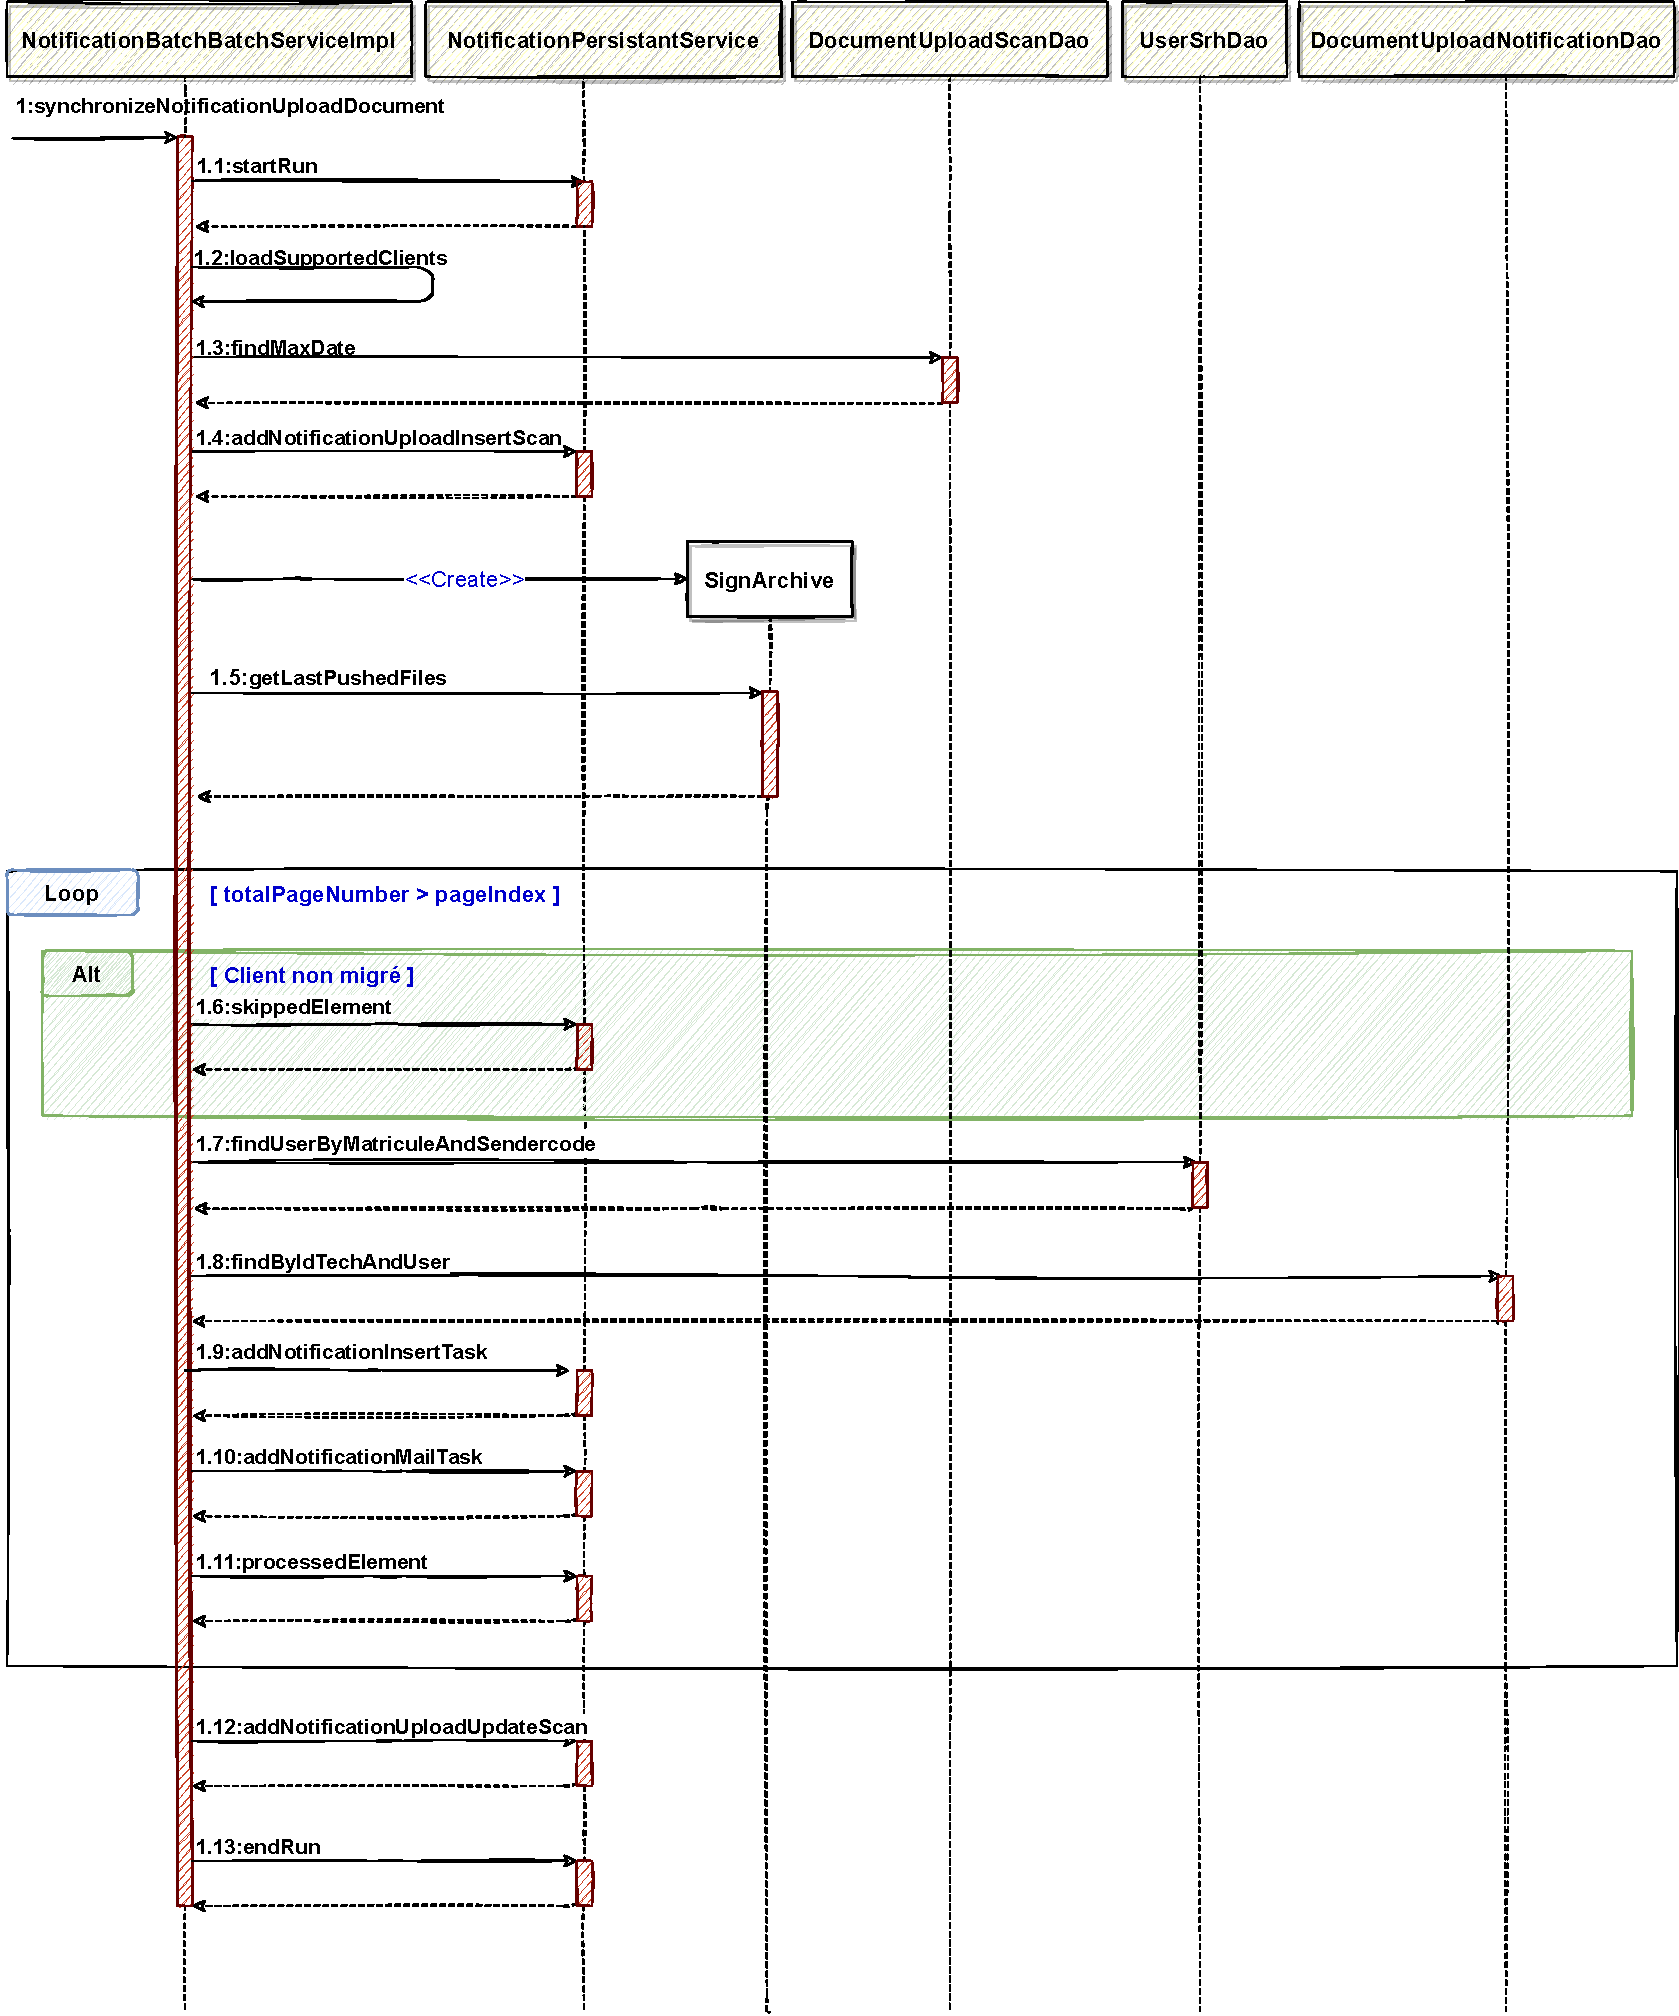
\includegraphics[width=\linewidth]{images/sec4/seq.pdf}
        \caption{Diagramme de séquence modélisant le processus d'envoi de notifications}
        \label{fig:seq}
    \end{center}
\end{figure}
\subsubsubsection*{Problématique et limites}
\begin{itemize}
    \item Mauvaise gestion des indices de recherche pour la méthode \lstinline|getLastPushedFiles|, ce qui conduit à boucler sur les documents déjà traités, et par conséquent à dépenser plus de ressources et de temps.\\

    \item L'appel Solr est couteuse en terme de temps, l'ancien mécanisme sollicite Solr pour chaque 20 documents (c'est-à-dire, si on a 1000 documents $\Longrightarrow$ on doit le solliciter 50 fois). 
    
    \item La réponse de Solr ne parvient pas à distinguer les clients migrés des clients non migrés, et l'ancien mécanisme prend en compte tous les documents, y compris ceux des clients qui n'ont pas encore migré. Le traitement de documents non pertinents exige un temps considérable.
\end{itemize}
\subsubsubsection*{La nouvelle approche}
Le système nouvellement conçu est une application autonome indépendante de l'application mère Arkevia, créée avec Spring Boot, une technologie qui facilite le développement d'applications basées sur Spring, et le framework Spring Batch pour orchestrer le traitement des notifications. Cela n'aurait pas été concevable sans recourir à des paradigmes de programmation avancés tels que le multithreading, qui permet la gestion et l'exécution d'un grand nombre d'instances de manière concurrente, ainsi que les concepts d'inversion de contrôle et d'injection de dépendances, qui facilitent la coordination et le contrôle de l'activité de l'application. Enfin, ce mécanisme a engendré des changements majeurs dans le processus d'extraction et l'exploitation des données, que nous allons expliquer dans la suite de cette section.\\

Le graphique suivant (voir figure \ref{fig:batch}) illustre de manière concrète la relation existant entre les différents composants impliqués dans le batcher lors de son exécution.
\begin{beware}[title=Note : ]
A noter que dans ce framework, lorsque l’on parle de batch on parle plus précisément de Job.
\end{beware}
    
\begin{figure}[!hbt]
    \begin{center}
        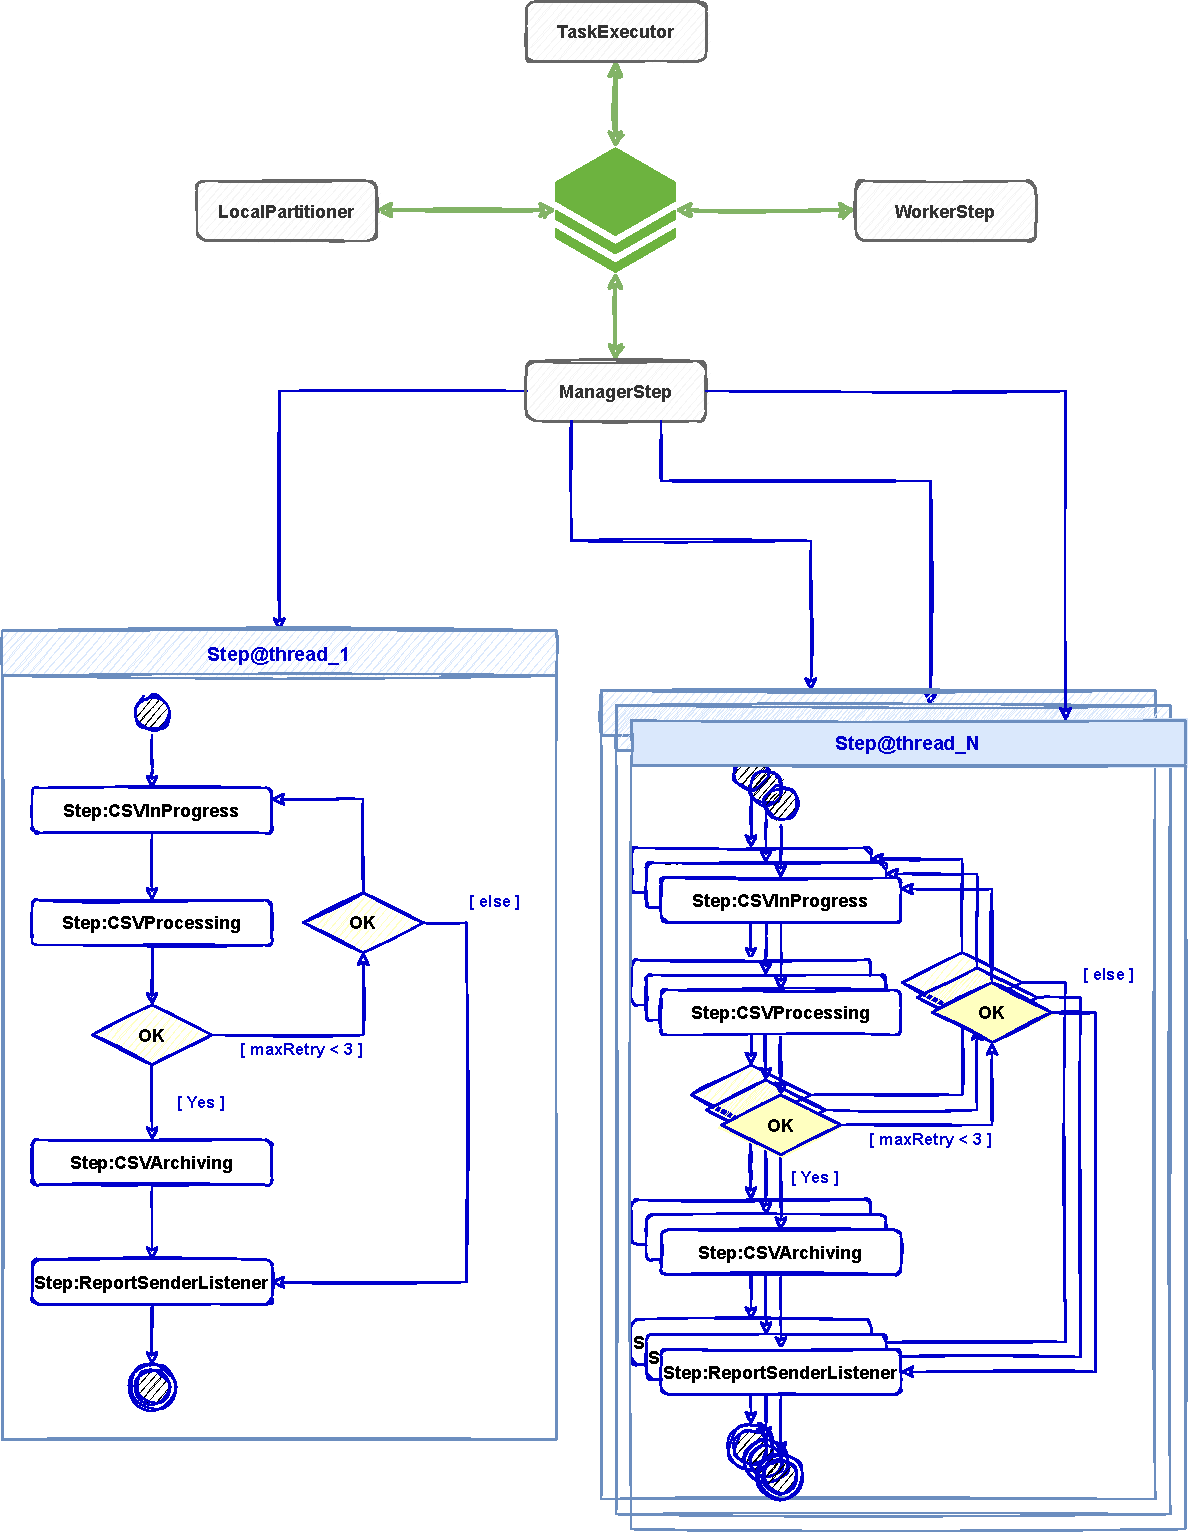
\includegraphics[width=\linewidth]{images/sec4/batchdiagram.pdf}
        \caption{Liens entre les divers composants impliqués dans le traitement par lots}
        \label{fig:batch}
    \end{center}
\end{figure}
\begin{itemize}
    \item \textbf{ManagerStep} : Ce composant permet de créer des copies des instances de step de flux basées sur une clé pour distribuer les données des fichiers provenant du Partitioner, également il se base sur le composant \textbf{taskExecutor} et principalement sur la valeur de \lstinline|maxPoolsize| pour définir le nombre maximum de threads à exécuter.
    \item \textbf{Partitioner} : est un composant qui permet de définir un ensemble de valeurs d'entrée sur une collection \lstinline|Map| pour chacun des fichiers existants. En d'autres termes, la logique pour diviser les tâches en threads respectifs va ici.
    \item \textbf{TaskExecutor} : est un JavaBean qui fournit une abstraction autour de l'instance \lstinline|java.util.concurrent.ThreadPoolExecutor| et l'expose en tant que Spring Bean. Grâce à ce composant, vous pouvez configurer le nombre de threads créés, le nombre de threads à conserver dans la file d'attente, le préfixe du thread, etc.
    \item \textbf{WorkerStep} : Représente le flux d'étapes qui seront appliquées et exécutées parallèlement pour accomplir le traitement d'un fichier donné.\\
\end{itemize}
\clearpage
\subsubsubsection*{Analyse du flux de données et traitement par lots}
L'application batch est planifiée par défaut pour s'exécuter automatiquement toutes les deux heures. Une fois le Job est lancé, le composant \textbf{Partitionneur} scanne le répertoire d'entrée afin de trouver des éventuels fichiers csv à traiter ;\\
À ce stade, il y a deux cas :

\begin{enumerate}
    \item Si le répertoire d'entrée \textbf{input} est vide, le programme scanne le répertoire \textbf{inprogress} pour vérifier s'il y a des fichiers qui ne sont pas traités correctement ou s'ils ont été interceptés lors d'une exécution antérieure ou encore bloqués pour un autre motif, dans ce contexte il y a deux hypothèses :
    \begin{enumerate}
        \item \underline{Le répertoire \textbf{inprogress} est vide}, dans ce cas le job se termine avec le statut \textbf{COMPLETED}.
        \item \underline{Le répertoire \textbf{inprogress} n'est pas vide}, dans ce cas le programme reprendra les fichiers CSV trouvés et les traitera une autre fois dans le cadre d'une politique de relance établie (fixée à 3 essais maximum).
    \end{enumerate}
    \item Si le répertoire d'entrée contient des fichiers, le programme créera des instances du Job (threads) pour traiter chaque fichier indépendamment ; le nombre de threads créés dépend de la valeur donnée au programme et du nombre de fichiers trouvés (pour altérer cette valeur, veuillez se référer à la propriété \lstinline|maxPoolSize| dans le fichier application.properties) ; si le nombre de fichiers dépasse le nombre maximum de threads autorisés, les fichiers restants seront ajoutés à la file d'attente (dès qu'un thread sera libre, il prendra en charge un fichier dans la file d'attente).\\
\end{enumerate}
Pour chaque thread lancé, le programme entreprend à différentes phases d'appliquer une série de validations aux fichiers associés afin de gérer efficacement le traitement et les cas de récupération en cas d'échec :
\begin{enumerate}
    \item La première phase est appelée \textbf{step:CSVInProgress}, elle permet de déplacer le fichier courant vers le répertoire \textbf{inprogress}, pour commencer son traitement.
    \item La phase successive est celle du traitement des fichiers CSV, elle constitue le cœur du processus batch et c'est dans cette phase que s'effectuent la lecture, la validation et la transformation des données, et finalement l'envoi des emails pour les données approuvées.
    \item Au terme de la deuxième phase, si le traitement du fichier s'est déroulé avec succès, le fichier sera acheminé à la dernière phase qui est celle de l'archivage du fichier. Dans le cas contraire, le fichier sera ignoré jusqu'à ce que le batch finisse le traitement des fichiers existants dans le répertoire d'entrée \textbf{input}, puis il le reprit ensuite pour un second traitement (fixée à trois tentatives maximum).\\
    \item Tout fichier ayant atteint ce stade d'archivage signifie que le fichier a été traité avec succès et il sera simplement déplacé vers le répertoire \textbf{done} et renommé selon le format suivant file\_name@date\_processing.csv.
    \item À la fin du Job, un email de contrôle incluant le statut de la dernière exécution, le nombre d'emails envoyés par client, ainsi qu'un fichier Excel contenant la liste des utilisateurs auxquels l'email de notification n'a pas été expédié, sera envoyé au responsable.
\end{enumerate}
\addcontentsline{toc}{subsection}{Conclusion}
\subsection*{Conclusion}
%%%%%%%%%%%%%%%%%%
